\RequirePackage{luatex85}
\documentclass[tikz]{standalone}
% Default preamble
\usepackage{pgfplots}
\pgfplotsset{compat=newest}
\usepgfplotslibrary{groupplots}
\usepgfplotslibrary{polar}
\usepgfplotslibrary{smithchart}
\usepgfplotslibrary{statistics}
\usepgfplotslibrary{dateplot}
\usepgfplotslibrary{ternary}
% Custom preamble from global variable:
\usetikzlibrary{patterns}
\usepackage{xcolor}
\definecolor{cred}{HTML}{ED1C24}
\definecolor{cgrey}{HTML}{7F7F7F}
\definecolor{cblue}{HTML}{00A2E8}
\definecolor{cgreen}{HTML}{22B14C}
\definecolor{cyellow}{HTML}{FFF200}
\definecolor{corange}{HTML}{EA7904}
\definecolor{cpurple}{HTML}{9100FC}
\definecolor{julia1}{HTML}{1F77B4}
\definecolor{julia2}{HTML}{FF7F0E}
\definecolor{julia3}{HTML}{2CA02C}
\definecolor{julia4}{HTML}{D62728}
\begin{document}
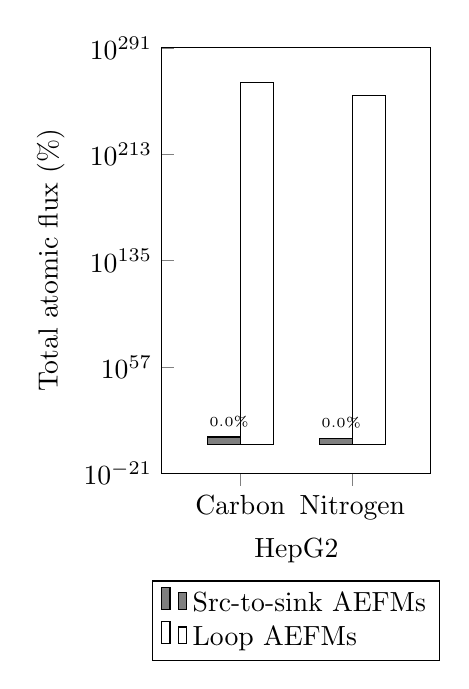
\begin{tikzpicture}
\begin{axis}[height={7cm}, width={5cm}, ybar = 0pt, ymode = log, xmajorgrids={false}, ymajorgrids={false}, xtick pos = bottom, ytick pos = left, bar width = 12pt, enlargelimits={0.1}, legend style={at={(0.5,-0.25)
}, anchor={north}, legend columns={1}, legend cell align={left}}, xmin={0.5}, xmax={2.5}, xtick={1,2}, xticklabels={Carbon,Nitrogen}, xlabel={HepG2}, ylabel={Total atomic flux (\%)}]
    \addplot[black, fill=cgrey]
        coordinates {
            (1,519561.2515154208)
            (2,63880.442045104)
        }
        ;
    \addplot[black, fill=none]
        coordinates {
            (1,4.785343315221769e265)
            (2,3.2389268396105266e256)
        }
        ;
    \legend{{Src-to-sink AEFMs},{Loop AEFMs}}
    \node [above,font=\tiny] at (axis cs: 0.9, 360000) {0.0\%};
    \node [above,font=\tiny] at (axis cs: 1.9, 85000) {0.0\%};
\end{axis}
\end{tikzpicture}
\end{document}
